%===============================================================================
% $Id: ifacconf.tex 7 2007-11-21 12:50:23Z jpuente $
% Template for IFAC meeting papers
% Copyright (c) 2007 International Federation of Automatic Control
%===============================================================================
\documentclass{ifacconf}
\usepackage[round]{natbib} % you should have natbib.sty
\usepackage{graphicx}      % include this line if your document contains figures

\usepackage{amsmath,amssymb}
\usepackage{url}
\usepackage{diffcoeff}
\usepackage{bm}
\usepackage{comment}

\usepackage{mathrsfs}
\usepackage{multirow}

\usepackage{caption, subfig}

\usepackage{xcolor,colortbl}

\newcommand{\mc}[2]{\multicolumn{#1}{c}{#2}}
% normal box
\newcommand{\sqboxs}{1.2ex}% the square size
\newcommand{\sqboxf}{0.6pt}% the border in \sqboxEmpty
\newcommand{\sqbox}[1]{\textcolor{#1}{\rule{\sqboxs}{\sqboxs}}}


% Math macros
\DeclareMathOperator*{\grad}{grad}
\DeclareMathOperator*{\Grad}{Grad}
\DeclareMathOperator*{\Div}{Div}
\renewcommand{\div}{\operatorname{div}}
\DeclareMathOperator*{\Hess}{Hess}
\DeclareMathOperator*{\curl}{curl}
\DeclareMathOperator{\Tr}{Tr}
\DeclareMathOperator{\Dom}{Dom}
\DeclareMathOperator*{\esssup}{ess\,sup}

\newcommand{\bbR}{\mathbb{R}}
\newcommand{\bbF}{\mathbb{F}}
\newcommand{\bbA}{\mathbb{A}}
\newcommand{\bbB}{\mathbb{B}}
\newcommand{\bbS}{\mathbb{S}}

\newcommand*{\norm}[1]{\ensuremath{\left\|#1\right\|}}
\newcommand{\where}{\qquad \text{where} \qquad}
\newcommand{\inner}[3][]{\ensuremath{\left\langle #2, \, #3 \right\rangle_{#1}}}
\newcommand{\bilprod}[2]{\left\langle \left\langle \, #1, #2 \, \right\rangle \right\rangle}
\newcommand{\pder}[2]{\ensuremath{\partial_{#2} #1}}
\newcommand{\dder}[2]{\ensuremath{\delta_{#2} #1}}
\newcommand{\secref}[1]{\S\ref{#1}}
\newcommand{\energy}[1]{\frac{1}{2} \int_{\Omega} \left\{ #1 \right\} \d\Omega}
\newcommand{\crmat}[1]{\ensuremath{\left[#1\right]_\times}}
\newcommand{\fenics}{\textsc{FEniCS}\xspace}
\newcommand{\firedrake}{\textsc{Firedrake}\xspace}

\DeclareMathOperator*{\argmax}{arg\,max}
\DeclareMathOperator*{\argmin}{arg\,min}


\newtheorem{proposition}{Proposition}
\newtheorem{proof}{Proof}
\newtheorem{remark}{Remark}
\newtheorem{hypothesis}{Hypothesis}
\newtheorem{assumption}{Assumption}
\newtheorem{conjecture}{Conjecture}

\def\onedot{$\mathsurround0pt\ldotp$}
\def\cddot{% two dots stacked vertically
	\mathbin{\vcenter{\baselineskip.67ex
			\hbox{\onedot}\hbox{\onedot}}%
}}

\makeatletter \renewcommand\d[1]{\ensuremath{%
		\;\mathrm{d}#1\@ifnextchar\d{\!}{}}}
\makeatother


\graphicspath{{./images/}}
%===============================================================================
\begin{document}
\begin{frontmatter}

\title{Mixed finite elements for port-Hamiltonian von K\'arm\'an beams} 
% Title, preferably not more than 10 words.


\author[UT]{Andrea Brugnoli}
\author[UT]{Stefano Stramigioli}
\author[UT]{Federico Califano}
\author[UT]{Ramy Rashad}
\author[ISAE]{Denis Matignon}
\address[UT]{University of Twente, Enschede (NL) \\
	a.brugnoli@utwente.nl, s.stramigioli@utwente.nl }

\address[ISAE]{ISAE-SUPAERO, Universit\'e de Toulouse, France.\\
	10 Avenue Edouard Belin, BP-54032, 31055 Toulouse Cedex 4. \\
	denis.matignon@isae.fr}

\begin{abstract}
A port-Hamiltonian formulation of von K\'arm\'an beams is presented. The variables selection lead to a non linear interconnection operator, while the constitutive laws are linear. The model can be readily discretized by exploiting a coenergy formulation and a mixed finite element method. The mixed formulation does not demand the $H^2$ regularity requirement typical of standard Galerkin discretization of thin structures. A numerical test is performed to assess the convergence rate of the solution. 
\end{abstract}

\begin{keyword}
Port-Hamiltonian systems, von K\'arm\'an beams, Mixed Finite Elements
\end{keyword}

\end{frontmatter}
%===============================================================================

\section{Introduction}

Linear elastic structures have been largely investigated into the port-Hamiltonian (pH) framework as well as the heat equation (consult for instance \cite{macchelli2004timo} for the Timoshenko beam, \cite{aoues2017modeling} for the Euler-Bernoulli beam, \cite{brugnoli2019mindlin,brugnoli2019kirchhoff} for thick and thin plates). Recently, more complicated models arising from fluid dynamics have also been considered \cite{cardoso2019port,cardoso2020swe,rashad2021port1,rashad2021port2,califano2021geometric,altmann2017}. \\


The Hamiltonian foundation of non-linear elasticity dates back to the late 80' \cite{simo1988}. However, the field of non-linear elasticity remains a largely unexplored topic in the pH framework. One fundamental non linear theory is the Von K\'arm\'an one, that applies for moderately large deformation of beams, plates and shells. This theory has puzzled mathematicians and physicists as the derivation of the model rely on some not well justified assumptions. Conditions under which this theory is actually applicable and will give reasonable results when solved are discussed in \cite{ciarlet1980,ciarlet1990}. Existence and uniqueness of solutions for the full dynamical problem were established in \cite{lagnese1991uniform} for one-dimensional beams and in \cite{puel1996} for plates. Since the full dynamical von K\'arman problem is conservative (see e.g. \cite{bilbao2015conservative}), a pH realization of this system exists. \\

The development of new models within the pH framework has been accompanied with an increased interest in numerical discretization methods, capable of retaining the main features of the distributed system in its finite-dimensional counterpart. Recently, it has become evident that there is a strict link between  discretization of port-Hamiltonian  systems and mixed finite elements \cite{cardoso2020pfem}. An example of this connection is given in \cite{kirby2015}, where a velocity-stress formulation for the wave dynamics is shown to be Hamiltonian and its mixed discretization preserves such a structure. \\

In this contribution, the von K\'arm\'an beam model is formulated as a pH system. The selection of energy variables will be such to make the Hamiltonian quadratic in these variables. As a consequence of this choice, the non linearities of the model are included in the interconnection operator, whereas the constitutive relations remain linear. The obtained model can be discretized using mixed finite element. To this aim, a weak formulation that does not demand for $H^2$ regularity for the vertical displacement (as in classical Galerkin discretizaiton of beams and plates, cf. \cite{gustafsson2018}) is obtained. A numerical test is carried out to evaluate the convergence rate of the discrete solution with respect to an analytical one. \\

The paper is organized as follows. In Section \ref{sec:vK_beams} the classical model for von K\'arm\'an beams is recalled. Then, a pH realization of the classical model is detailed in \secref{sec:pHmodel}. The mixed finite elements discretization strategy is discussed in \secref{sec:mfem}. In Sec. \ref{sec:num_test} a numerical convergence test is performed to assess the rate of convergence of the solution.



\section{Von K\'arm\'an beams}\label{sec:vK_beams}


The classical von-K\'arm\'an beam model is presented in \cite[Chapter 4]{reddy2010introduction}. Under the hypothesis of isotropic material, the extensional-bending stiffness is zero when the $x$-axis is taken along the geometric centroidal axis. With this assumption, the problem, defined on an interval $\Omega = [0, L]$, takes the following form

\begin{equation}\label{eq:class}
	\begin{aligned}
		\rho A \ddot{u} &= \partial_x n_{xx}, \\
		\rho A \ddot{w} &= -\partial^2_{xx} m_{xx} + \partial_x(n_{xx} \partial_x w),
	\end{aligned} 
\end{equation}
together with the stresses and strains expressions
\begin{equation}
	\begin{aligned}
		n_{xx} &= EA \varepsilon_{xx}, \\
		\varepsilon_{xx} &= \partial_x u + 1/2 (\partial_x w)^2, \\
	\end{aligned} \quad
	\begin{aligned}
		m_{xx} &= EI \kappa_{xx}, \\
		\kappa_{xx} &=\partial^2_{xx} w. \\
	\end{aligned} 
\end{equation}
Variable $u$ is the horizontal displacement, $w$ is the vertical displacement, $n_{xx}$ is the axial stress resultant and $m_{xx}$ is the bending stress resultant. The coefficients $\rho, A, E, I$ are the mass density, the cross section, the Young modulus and the second moment of area.

The total energy of the model (Hamiltonian functional)
\begin{equation}
	H = \frac{1}{2} \int_{\Omega}\left\{\rho A (\dot{u}^2 + \dot{w}^2) + n_{xx} \varepsilon_{xx} + m_{xx} \kappa_{xx} \right\} \d\Omega,
\end{equation}
consists of the kinetic energy and both membrane and bending deformation energies.
This model proves conservative, see \cite{bilbao2015conservative}. Indeed, this implies that a port-Hamiltonian realization of the system exists. We shall demonstrate how to construct a port-Hamiltonian realization, equivalent to \eqref{eq:class}.


\section{The equivalent port-Hamiltonian realization}\label{sec:pHmodel}
To find a suitable port-Hamiltonian system, we first select a set of new energy variables to make the Hamiltonian functional quadratic
\begin{equation}\label{eq:energies}
	\alpha_u = \rho A \dot{u}, \quad \alpha_\varepsilon = \varepsilon_{xx}, \quad \alpha_w = \rho A \dot{w}, \quad \alpha_\kappa = \kappa_{xx}.
\end{equation}
The energy is quadratic in these variables
\begin{equation}
	H = \frac{1}{2} \int_{\Omega} \left\{\frac{\alpha_u^2 + \alpha_w^2}{\rho A} + EA \varepsilon_{xx}^2 + EI \kappa_{xx}^2 \right\} \d{\Omega}.
\end{equation}
By computing the variational derivative of the Hamiltonian, one obtains the so-called co-energy variables:
\begin{equation}\label{eq:coenergies}
	\begin{aligned}
	e_u &:= \delta_{\alpha_u} H = \dot{u}, \\
	e_w &:= \delta_{\alpha_w} H = \dot{w}, \\
	\end{aligned} \qquad 
\begin{aligned}
	e_\varepsilon &:= \delta_{\alpha_\varepsilon} H = n_{xx}, \\ e_\kappa &:= \delta_{\alpha_\kappa} H = m_{xx}.
\end{aligned}
\end{equation}
Before stating the final formulation, consider the unbounded operator operator $\mathcal{C}(w)(\cdot): L^2(\Omega) \rightarrow L^2(\Omega)$, that acts as follows
\begin{equation}
	\mathcal{C}(w)(\cdot ) = \partial_x(\cdot \; \partial_x w).
\end{equation}
\begin{proposition}\label{prop:adjC}
	The formal adjoint of the $\mathcal{C}(w)(\cdot)$ is given by
	\begin{equation}
		\mathcal{C}(w)^*(\cdot) = -\partial_x (\cdot) \partial_x(w).
	\end{equation}
\end{proposition}
\begin{proof}
	Consider a smooth scalar fields with compact support  $\psi \in C^\infty_0(\Omega)$ and $\xi \in C^\infty_0(\Omega)$. The formal adjoint of $\mathcal{C}(w)(\cdot)$ satisfies the relation
	\begin{equation}
		\inner[\Omega]{\psi}{\mathcal{C}(w)(\xi)} = \inner[\Omega]{\mathcal{C}(w)^*(\psi)}{\xi},
	\end{equation}
	where $\inner[\Omega]{f}{g} = \int_\Omega f g \d{\Omega}$.
	The proof follows from the computation
	\begin{equation}
		\begin{aligned}
			\inner[\Omega]{\psi}{\mathcal{C}(w)(\xi)} &= \inner[\Omega]{\psi}{\partial_x(\xi \, \partial_x w)}, \\
			&= \inner[\Omega]{-\partial_x \psi}{\xi \partial_x w}, \\
			&= \inner[\Omega]{-\partial_x \psi \, \partial_x w}{\xi}.
		\end{aligned} 
	\end{equation}
	This means that
	\begin{equation}
		\mathcal{C}(w)^*(\cdot) = -\partial_x (\cdot) \partial_x w,
	\end{equation}
	leading to the final result.
\end{proof}

The pH realization is then given by the following system
\begin{equation}\label{eq:pHsys}
	\frac{\partial}{\partial t}
	\begin{pmatrix}
		\alpha_u \\
		\alpha_\varepsilon \\
		\alpha_w \\
		\alpha_\kappa
	\end{pmatrix} = 
	\begin{bmatrix}
		0 & \partial_x & 0 & 0 \\
		\partial_x & 0 & (\partial_x w) \, \partial_x & 0 \\
		0 & \partial_x(\cdot \, \partial_x w) & 0 & -\partial_{xx}^2 \\
		0 & 0 & \partial_{xx}^2 & 0 \\ 
	\end{bmatrix}
	\begin{pmatrix}
		e_u \\
		e_\varepsilon \\
		e_w \\
		e_\kappa 
	\end{pmatrix}.
\end{equation}
The second line of system \eqref{eq:pHsys} represents the time derivative of the membrane strain. To close the system, variable $w$ has to be accessible. For this reason, its dynamics has to be included. The augmented system reads
\begin{equation}\label{eq:pHsys_aug}
	\frac{\partial}{\partial t}
	\begin{pmatrix}
		\alpha_u \\
		\alpha_\varepsilon \\
		\alpha_w \\
		\alpha_\kappa \\
		w \\
	\end{pmatrix} = 
	\underbrace{\begin{bmatrix}
			0 & \partial_x & 0 & 0 & 0\\
			\partial_x & 0 & (\partial_x w) \, \partial_x & 0 & 0 \\
			0 & \partial_x(\cdot \, \partial_x w) & 0 & -\partial_{xx}^2 & -1 \\
			0 & 0 & \partial_{xx}^2 & 0 & 0 \\ 
			0 & 0 & 1 &  & 0 \\
	\end{bmatrix}}_{\mathcal{J}}
	\begin{pmatrix}
		e_u \\
		e_\varepsilon \\
		e_w \\
		e_\kappa \\
		\delta_w H  \\
	\end{pmatrix}.
\end{equation}
The operator $\mathcal{J}$ is formally skew-adjoint. If only the kinetic and deformation energies are considered, it holds $\delta_{w} H~=~0$. In general this terms allows accommodating for other potentials, for example the gravitational one. Suitable boundary variables are then obtained considering the power balance
\begin{equation}
	\dot{H} = \inner[\partial\Omega]{e_u}{e_\varepsilon} + \inner[\partial\Omega]{e_w}{e_\varepsilon \partial_x w -\partial_x e_\kappa} + \inner[\partial\Omega]{\partial_x e_w}{e_\kappa}.
\end{equation}

The boundary conditions are consistent with the ones assumed in \cite{puel1996} for deriving a global existence result for this model.


\section{Mixed finite element discretization}\label{sec:mfem}
To perform the numerical discretization, the constitutive relations are first incorporated in the dynamics. The link between the energy variables \eqref{eq:energies} and the conergy variables \eqref{eq:coenergies} is given by the linear transformation

\begin{equation}\label{eq:e2alpha}
	\begin{pmatrix}
		\alpha_u \\ \alpha_\varepsilon \\ \alpha_w \\ \alpha_\kappa
	\end{pmatrix} =
	\begin{bmatrix}
	\rho A & 0 & 0 & 0 \\
	0 & C_a & 0 & 0 \\
	0 & 0 & \rho A & 0 \\
	0 & 0 & 0 & C_b
	\end{bmatrix}
	\begin{pmatrix}
		e_u \\ e_\varepsilon \\ e_w \\ e_{\kappa}
	\end{pmatrix},
\end{equation}
where $C_a = (EA)^{-1}$ and $C_b = (EI)^{-1}$ are the axial and bending compliances respectively. A pure coenergy formulation can then be employed once \eqref{eq:e2alpha} is plugged into \eqref{eq:pHsys_aug}

\begin{equation}\label{eq:pHaug_e}
	\begin{pmatrix}
		\rho A \dot{e}_u \\
		C_a \dot{e}_\varepsilon \\
		\rho A \dot{e}_w \\
		C_b \dot{e}_\kappa \\
		\dot{w} \\
	\end{pmatrix} = 
	\begin{bmatrix}
		0 & \partial_x & 0 & 0 & 0\\
		\partial_x & 0 & \partial_x w \, \partial_x & 0 & 0 \\
		0 & \partial_x(\cdot \, \partial_x w) & 0 & -\partial_{xx}^2 & -1 \\
		0 & 0 & \partial_{xx}^2 & 0 & 0 \\ 
		0 & 0 & 1 &  & 0 \\
	\end{bmatrix}
	\begin{pmatrix}
		e_u \\
		e_\varepsilon \\
		e_w \\
		e_\kappa \\
		\delta_w H \\
	\end{pmatrix}.
\end{equation}

To derive the discrete system, first \eqref{eq:pHaug_e} is put into weak form. To this aim the test functions $(\psi_u,\, \psi_\varepsilon,\, \psi_w,\, \psi_\kappa,\, \psi)$ are introduced. For sake of simplicity, no dependency between the displacements and the energy is considered, i.e. $\delta_w H=0$:
\begin{equation}
	\begin{aligned}
	\inner[\Omega]{\psi_u}{\rho A \, \dot{e}_u} &= \inner[\Omega]{\psi_u}{\partial_x e_\varepsilon}. \\
	\inner[\Omega]{\psi_\varepsilon}{C_a \, \dot{e}_\varepsilon} &= \inner[\Omega]{\psi_\varepsilon}{\partial_x e_u} + \inner[\Omega]{\psi_\varepsilon}{(\partial_x w) \, \partial_x e_w}, \\
	\inner[\Omega]{\psi_w}{\rho A\dot{e}_w} &= \inner[\Omega]{\psi_w}{\partial_x(e_\varepsilon \partial_x w)} - \inner[\Omega]{\psi_w}{\partial^2_{xx} e_\kappa}, \\
	\inner[\Omega]{\psi_\kappa}{C_b \, \dot{e}_\kappa} &= \inner[\Omega]{\psi_\kappa}{\partial^2_{xx} e_w}, \\
	\inner[\Omega]{\psi}{\dot{w}} &= \inner[\Omega]{\psi}{e_w}. \\
	\end{aligned}
\end{equation}

Then the integration by parts is performed on the first, third and fourth line. This choice is such to retain the skew-symmetric structure at the discrete level and to lower the regularity requirement for the finite elements \cite[Chap. 8]{brugnoli2020thesis}. The weak formulation then looks for $(e_u, e_w, e_\kappa, w) \in H^1(\Omega), \, e_\varepsilon \in L^2(\Omega)$
such that the following system
\begin{equation}\label{eq:weak_form}
	\begin{aligned}
		\inner[\Omega]{\psi_u}{\rho A \, \dot{e}_u} &= -\inner[\Omega]{\partial_x \psi_u}{ e_\varepsilon} +  \inner[\partial\Omega]{\psi_u}{e_\varepsilon}. \\
		\inner[\Omega]{\psi_\varepsilon}{C_a \, \dot{e}_\varepsilon} &= \inner[\Omega]{\psi_\varepsilon}{\partial_x e_u} + \inner[\Omega]{\psi_\varepsilon}{\partial_x w \, \partial_x e_w}, \\
		\inner[\Omega]{\psi_w}{\rho A\dot{e}_w} &= -\inner[\Omega]{\partial_x \psi_w \partial_x w}{e_\varepsilon} + \inner[\Omega]{\partial_{x} \psi_w}{\partial_{x} e_\kappa} \\
		&\quad +\inner[\partial\Omega]{\psi_w}{e_\varepsilon \partial_x w - \partial_x e_\kappa}, \\
		\inner[\Omega]{\psi_\kappa}{C_b \, \dot{e}_\kappa} &= - \inner[\Omega]{\partial_{x} \psi_\kappa}{\partial_{x} e_w} + \inner[\partial\Omega]{\psi_\kappa}{\partial_x e_w}, \\
		\inner[\Omega]{\psi}{\dot{w}} &= \inner[\Omega]{\psi}{e_w}. \\
	\end{aligned}
\end{equation}
holds $\forall (\psi_u, \psi_w, \psi_\kappa, \psi) \in H^1(\Omega), \, \forall \psi_\varepsilon \in L^2(\Omega)$. For the boundary terms, the following notation has been used
\begin{equation*}
	\inner[\partial\Omega]{f}{g} = f g \vert_{0}^L = f(L)g(L) - f(0)g(0).
\end{equation*} 
In this formulation, the boundary axial forces $e_\varepsilon\vert_{0}^L$, vertical forces $e_\varepsilon\partial_x w - \partial_x e_\kappa\vert_{0}^L$ and  rotations $\partial_x e_w\vert_{0}^L$ are enforced weakly. To obtain the associated finite-dimensional system, the following Galerkin approximation is considered 
\begin{equation}\label{eq:Gal_appr}
\begin{aligned}
	e_u^h &= \sum_{i=1}^{n_u} \xi_u^i(x) e_u^i(t), \\
	e_\varepsilon^h &= \sum_{i=1}^{n_\varepsilon} \xi_\varepsilon^i(x) e_\varepsilon^i(t), \\
	e_w^h &= \sum_{i=1}^{n_w} \xi_w^i(x) e_w^i(t), \\
	e_\kappa^h &= \sum_{i=1}^{n_\kappa} \xi_\kappa^i(x) e_\kappa^i(t), \\
	w^h &= \sum_{i=1}^{n_w} \xi_w^i(x) w^i(t), \\
\end{aligned} \qquad 
\begin{aligned}
	\psi_u^h &= \sum_{i=1}^{n_u} \xi_u^i(x) \psi_u^i, \\
	\psi_\varepsilon^h &= \sum_{i=1}^{n_\varepsilon} \xi_\varepsilon^i(x) \psi_\varepsilon^i, \\
	\psi_w^h &= \sum_{i=1}^{n_w} \xi_w^i(x) \psi_w^i, \\
    \psi_\kappa^h &= \sum_{i=1}^{n_\kappa} \xi_\kappa^i(x) \psi_\kappa^i, \\
	\psi^h &= \sum_{i=1}^{n_w} \xi_w^i(x) \psi^i. \\
\end{aligned}
\end{equation}
Notice that $w, \, e_w$ are discretized using the same test functions 
$\xi_w^i(x)$. Plugging \eqref{eq:Gal_appr} into \eqref{eq:weak_form}, the following-finite dimensional system is obtained

\begin{equation}\label{eq:findimSys}
\begin{pmatrix}
	\mathbf{M}_u \dot{\mathbf{e}}_u \\
	\mathbf{M}_\varepsilon \dot{\mathbf{e}}_\varepsilon \\
	\mathbf{M}_w \dot{\mathbf{e}}_w \\
	\mathbf{M}_\kappa \dot{\mathbf{e}}_\kappa \\
	 \dot{\mathbf{w}}
\end{pmatrix} = 
\begin{bmatrix}
	\mathbf{0} & -\mathbf{D}_{\varepsilon u}^\top & \mathbf{0} & \mathbf{0}  \\
	\mathbf{D}_{\varepsilon u} & \mathbf{0} & \mathbf{D}_{\varepsilon w}(\mathbf{w}) & \mathbf{0}  \\
	\mathbf{0} & -\mathbf{D}_{\varepsilon w}^\top(\mathbf{w}) & \mathbf{0} & \mathbf{D}_{w \kappa} \\
	\mathbf{0} & \mathbf{0} & -\mathbf{D}_{w \kappa}^\top & \mathbf{0}  \\
	\mathbf{0} & \mathbf{0} & \mathbf{I} & \mathbf{0} \\ 
\end{bmatrix}
\begin{pmatrix}
	\mathbf{e}_u \\
	\mathbf{e}_\varepsilon \\
	\mathbf{e}_w \\
	\mathbf{e}_\kappa \\
\end{pmatrix}.
\end{equation}
The boundary terms have been omitted for simplicity. The fifth column disappear because $\delta_w H=0$. The mass matrices are defined as follows
\begin{equation}
	\begin{aligned}
	M_u^{ij} &= \inner[\Omega]{\xi_u^i}{\rho A \xi_u^j}, \\
	M_\varepsilon^{ij} &= \inner[\Omega]{\xi_\varepsilon^i}{C_a \xi_\varepsilon^j}, 
	\end{aligned} \qquad 
	\begin{aligned}
	M_w^{ij} &= \inner[\Omega]{\xi_w^i}{\rho A \xi_w^j}, \\
	M_\kappa^{ij} &= \inner[\Omega]{\xi_\kappa^i}{C_b \xi_\kappa^j}.
	\end{aligned}
\end{equation}

The interconnection matrices are given by 
\begin{equation}
	\begin{aligned}
	D_{\varepsilon u}^{ij} &= \inner[\Omega]{\xi_\varepsilon^i}{\partial_x \xi_u^j}, \\
	D_{\varepsilon w}^{ij}(\mathbf{w}) &= \inner[\Omega]{\xi_\varepsilon^i}{ \sum_{k=1}^{n_w} \partial_x \xi_w^k(x) w^k(t) \partial_x \xi_w^j}, \\
	D_{w \kappa}^{ij} &= \inner[\Omega]{\partial_x \xi_w^i}{\partial_x \xi_\kappa^j}.
	\end{aligned}
\end{equation}


For what concerns the choice of the underlying finite elements, a simple selection conforming to the weak form \eqref{eq:weak_form} is given by continuous Galerkin to discretize the space $H^1(\Omega)$ and discontinuous Galerkin for the space $L^2(\Omega)$. Consider an interval mesh $\mathcal{I}_h$ with elements $E$. The space of polynomials of order $k$ on a mesh cell is denoted by $P_k$. The following conforming families of finite elements are selected for this problem:

\begin{equation}
	\begin{aligned}
		H^1_h(\Omega) &= \left\{v_h \in H^1(\Omega)\vert \forall E \in \mathcal{I}_h, \; v_h\vert_E \in P_k \right\}, \\
		L^2_h(\Omega) &= \left\{u_h \in L^2(\Omega)\vert \forall E \in \mathcal{I}_h, \; u_h\vert_E \in P_{k-1} \right\}.
	\end{aligned}
\end{equation}

The space $H^1_h$ corresponds to the space of continous Galerkin elements of order $k$, whereas $L^2_h$ corresponds to the space of discontinuous Galerkin elements of order $k-1$. This choice guarantees that $\partial_x H^1_h(\Omega) \subset L^2_h(\Omega)$. So the discrete weak formulation becomes: find $(e_u^h, e_w^h, e_\kappa^h, w^h) \in H^1_h(\Omega), \, e_\varepsilon^h \in L_h^2(\Omega)$
such that system \eqref{eq:weak_form} holds $\forall (\psi_u^h, \psi_w^h, \psi_\kappa^h, \psi^h) \in H^1_h(\Omega), \, \forall \psi_\varepsilon^h \in L^2_h(\Omega)$.

\section{Numerical test}\label{sec:num_test}

Consider the following analytical solution for the axial and vertical displacement

\begin{equation}\label{eq:analytical}
	\begin{aligned}
		u^{\text{ex}} &= x^3[1-(x/L)^3] \sin(2 \pi t), \\
		w^{\text{ex}} &= \sin(\pi x/L)\sin(2 \pi t), \\
	\end{aligned}
\end{equation}
together with the boundary conditions
\begin{equation}
u\vert_0^L = 0, \quad w\vert_0^L =0, \quad m_{xx}\vert_{0}^L=0.
\end{equation}
For $u$ and $w$ given in \eqref{eq:analytical} to be the solution of \eqref{eq:class}, appropriate forcing term have to be introduced. These are given by 
\begin{equation}\label{eq:forcing}
	\begin{aligned}
		f_u &= \rho A \partial_{tt}^2 u^{\text{ex}} - \partial_x n_{xx}^{\text{ex}}, \\
		f_w &= \rho A \partial_{tt}^2 w^{\text{ex}} + \partial_{xx}^2 m_{xx}^{\text{ex}} - \partial_x(n_{xx}^{\text{ex}} \partial_x w^{\text{ex}}), \\
	\end{aligned}
\end{equation}

The numerical values of the parameters for the simulation are reported in Table \ref{tab:par}. The Firedrake library (\cite{rathgeber2017firedrake}) is used to generate the matrices. To integrate the equations in time a Crank-Nicholson scheme is employed. The time step is set to $\Delta t = h/(2 \pi)$ to have the same impact of the time discretization error with respect to the spatial error. The final time is set to one $t_f = 1 [\textrm{s}]$. The non-linear system is solved using Newton-Krylov iterations with a line search and direct factorization of the linear system.  \\

To measure the convergence rate,  suitable norms have to be introduced. 
Let $\mathcal{X}$ be a Hilbert space, and $t_f$ a positive real number. We denote by $L^\infty([0, t_f]; \mathcal{X})$ or $L^\infty(\mathcal{X})$ the space of functions $f: [0, t_f] \rightarrow \mathcal{X}$ for which the time-space norm $||\cdot||_{L^\infty([0, t_f]; \mathcal{X})}$ satisfies
\[
||f||_{L^\infty([0, t_f]; \mathcal{X})} = \esssup_{t \in [0,t_f]} ||f||_{\mathcal{X}} < \infty.
\]

To compute the $L^\infty (\mathcal{X})$ space-time dependent norm from the numerical results, the discrete norm $L^\infty_{\Delta t} (\mathcal{X})$ is used
\[
||\cdot ||_{L^\infty (\mathcal{X})} \approx || \cdot ||_{L^\infty_{\Delta t} (\mathcal{X})} = \max_{t \in t_i} ||\cdot||_{\mathcal{X}},
\]
where $t_i$ are the discrete simulation instants. The Hilbert space $\mathcal{X}$ depends on the regularity of the considered variable. For variables $(e_u,\, e_w,\, e_\kappa,\, w)$ the error is measured in the $L^\infty_{\Delta t}(H^1)$ norm, whereas for $e_\varepsilon$ is measured using the $L^\infty_{\Delta t}(L^2)$ norm. The simulation results are reported in Fig. \ref{fig:error}. It can be noticed that all variables converge at rate given by the polynomial degree $k$. For variable $e_\kappa$ a superconvergent trend can be observed for case $k=1$ (cf. Fig \ref{fig:err_e_kap}). The numerical solutions for the different variables is plotted in Fig. \ref{fig:plot}.


\begin{table}[h]
	\centering
	\begin{tabular}{ccccc}
		\hline 
		\multicolumn{5}{c}{Beam parameters} \\ 
		\hline 
		$E$ & $\rho$ & $L$  & $A$ & $I$ \\
		70 $[\textrm{kPa}]$ & $2700\; [\textrm{kg}/\textrm{m}^3]$ & 1 $[\textrm{m}]$ &  0.01 $[\textrm{m}^2]$ & $8.3 \; 10^{-6} \, [\textrm{m}^4]$\\ 
		\hline 
	\end{tabular} 
	\captionsetup{width=0.95\linewidth}
	\vspace{1mm}
	\captionof{table}{Physical parameters for the beam.}
	\label{tab:par}
\end{table}

\begin{figure}[ht]%
	\centering
	\subfloat[][$L^\infty_{\Delta t} (H^1)$ error for $e_u$]{%
		\label{fig:err_e_u}%
		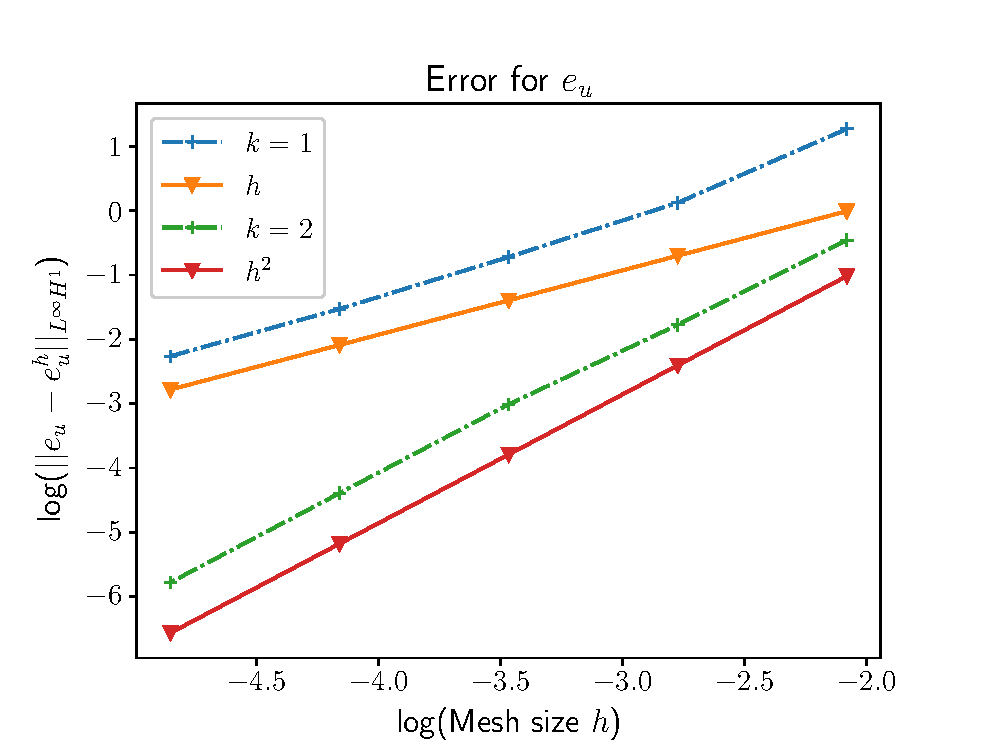
\includegraphics[width=0.48\columnwidth]{u_dot.eps}}%
	\hspace{8pt}%
	\subfloat[][$L^\infty_{\Delta t} (L^2)$ error for $e_\varepsilon$]{%
		\label{fig:err_e_eps}%
		\includegraphics[width=0.48\columnwidth]{n_xx.eps}} \\
	\subfloat[][$L^\infty_{\Delta t} (H^1)$ error for $e_w$]{%
		\label{fig:err_e_w}%
		\includegraphics[width=0.48\columnwidth]{w_dot.eps}}%
	\hspace{8pt}%
	\subfloat[][$L^\infty_{\Delta t} (H^1)$ error for $e_\kappa$]{%
		\label{fig:err_e_kap}%
		\includegraphics[width=0.48\columnwidth]{m_xx.eps}} \\
	\subfloat[][$L^\infty_{\Delta t} (H^1)$ error for $w$]{%
		\label{fig:err_e_disp}%
		\includegraphics[width=0.48\columnwidth]{w.eps}}%
	\caption{Error trend for the different variables}%
	\label{fig:error}%
\end{figure}

\begin{figure}[ht]%
	\centering
	\subfloat[][Numerical solution $e_u^h$]{%
		\label{fig:plot_e_u}%
		\includegraphics[width=0.48\columnwidth]{plot_e_u_cropped.eps}}%
	\hspace{8pt}%
	\subfloat[][Numerical solution for $e_\varepsilon^h$]{%
		\label{fig:plot_e_eps}%
		\includegraphics[width=0.48\columnwidth]{plot_e_eps_cropped.eps}} \\
	\subfloat[][Numerical solution $e_w^h$]{%
		\label{fig:plot_e_w}%
		\includegraphics[width=0.48\columnwidth]{plot_e_w_cropped.eps}}%
	\hspace{8pt}%
	\subfloat[][Numerical solution $e_\kappa^h$]{%
		\label{fig:plot_e_kap}%
		\includegraphics[width=0.48\columnwidth]{plot_e_kap_cropped.eps}} \\
	\subfloat[][Numerical solution $w^h$]{%
		\label{fig:plot_e_disp}%
		\includegraphics[width=0.48\columnwidth]{plot_w_cropped.eps}}%
	\caption{Computed numerical solution for $h=2^{-7}$ and $k=2$ for the different variables}%
	\label{fig:plot}%
\end{figure}

\section{Conclusion}

In this contribution, a pH model for von K\'arm\'an beams is detailed. The resulting system of equations is then discretized using mixed finite elements. The validity of discretized model is assessed by comparison with an analytical solution. This demonstrates how pH formulations can be used in relevant non linear models arising from engineering. A natural outlook is the extension of this formulation to the two-dimensional case \cite{brugnoli2021enoc}. \\

The analysis of this model under a control theoretic perspective represents another interesting development. The numerical discrete model can be used to construct model based controllers.


\bibliography{biblio_LHMNC}             % bib file to 
\appendix

      
                                                          % in the appendices.
\end{document}
